%%%% using 'arara' 4.0
% arara: xelatex: {synctex: yes, interaction: nonstopmode}
% arara: bibtex
% arara: xelatex: {synctex: yes, interaction: nonstopmode}
% arara: xelatex: {synctex: yes, interaction: nonstopmode}

%% arara: indent: {overwrite: yes}

% arara: clean: { extensions: [bcf, cod, blg, lof, lot, out, toc, xml, bak0 ] }

\documentclass[review]{elsarticle}

% Figures Links, mittig und rechts platzieren
\usepackage[export]{adjustbox}
\usepackage{caption}
\usepackage{subcaption}
\usepackage{amsmath}

\usepackage{enumerate}

% prevents that appendices are moved behind references
\usepackage{placeins}

\usepackage[nolist]{acronym}

\usepackage{longtable}
\usepackage{booktabs}
\usepackage{multirow}
\usepackage{float}

% https://tex.stackexchange.com/questions/165115/getting-not-defining-perthousnad-and-not-defining-micro-when-compiling-beamer
\usepackage{textcomp}

\graphicspath{{../03_figures/results/}{./}{../03_figures/data/}}

% enable linking to subsubsection
\setcounter{secnumdepth}{3}

% various symbols, e.g. \degree
\usepackage{gensymb}

\usepackage[hidelinks]{hyperref}

\usepackage{lineno}
\modulolinenumbers[5]

% set autoref abbr for appendix
\newcommand*{\Appendixautorefname}{appendix}

\journal{Journal "Remote Sensing of Environment"}

% line breaks in table cells
\newcommand{\specialcell}[2][l]{%
  \begin{tabular}[#1]{@{}l@{}}#2\end{tabular}}

% tilde
\newcommand{\mytilde}{\raise.17ex\hbox{$\scriptstyle\mathtt{\sim}$}}

%% APA style
\bibliographystyle{model5-names}\biboptions{authoryear}

\begin{document}

\begin{frontmatter}

	\title{Modeling defoliation as a proxy for tree health: A case study using machine-learning and hyperspectral remote sensing data}

	%% Group authors per affiliation:
	\author[FSU]{Patrick Schratz}
	\cortext[mycorrespondingauthor]{Corresponding author}
	\ead{patrick.schratz@uni-jena.de}

	\author[FSU]{Jannes Muenchow}
	\author[NEIKER]{Eugenia Iturritxa}
	\author[LMU]{Bernd Bischl}
	\author[FSU]{Alexander Brenning}

	\address[FSU]{Department of Geography, GIScience group, Grietgasse 6, 07743, Jena, Germany}
	\address[NEIKER]{NEIKER, Granja Modelo –Arkaute, Apdo. 46, 01080 Vitoria-Gasteiz, Arab, Spain}
	\address[LMU]{Department of Statistics, Chair for computational Statistics, Ludwig-Maximilian University Munich, Germany}

	\begin{abstract}

	\end{abstract}

	\begin{keyword}
		hyperspectral imagery \sep forest health modeling \sep machine-learning \sep feature-selection  \sep model comparison
	\end{keyword}

\end{frontmatter}

\linenumbers

% längste Abkürzung steht hier!!! in eckigen Klammern
\begin{acronym}[AUROC]

	% geringerer Zeilenabstand
	%\setlength{\itemsep}{-\parsep}
	\acro{AGB}{Above-Ground Biomass}
	\acro{ALS}{airborn laser scanning}
	\acro{ANN}{Artificial Neural Network}
	\acro{AUROC}{Area Under the Receiver Operating Characteristics Curve}
	\acro{BRT}{Boosted Regression Trees}
	\acro{CART}{Classification and Regression Trees}
	\acro{CNN}{convolutional neural networks}
	\acro{CV}{cross-validation}
	\acro{DAP}{digital aerial photogrammetry}
	\acro{ENM}{Environmental Niche Modeling}
	\acro{FPR}{False Positive Rate}
	\acro{FFS}{forward feature-selection}
	\acro{FS}{feature-selection}
	\acro{GAM}{Generalized Additive Model}
	\acro{GBM}{Gradient Boosting Machine}
	\acro{GLM}{Generalized Linear Model}
	\acro{ICGC}{Institut Cartografic i Geologic de Catalunya}
	\acro{IQR}{Interquartile Range}
	\acro{MARS}{Multivariate Adaptive Regression Splines}
	\acro{MEM}{Maximum Entropy Model}
	\acro{ML}{Machine-Learning}
	\acro{NDII}{Normalized Difference Infrared Index}
	\acro{NIR}{Near-Infrared}
	\acro{NRI}{Normalized Ratio Index}
	\acro{OLS}{ordinary least squares}
	\acro{LiDAR}{light detection and ranging}
	\acro{LOWESS}{Locally Weighted Scatter Plot Smoothing}
	\acro{PISR}{Potential Incoming Solar Radiation}
	\acro{PLS}{partial least-squares}
	\acro{RBF}{Radial Basis Function}
	\acro{RF}{Random Forest}
	\acro{RMSE}{Root Mean Square Error}
	\acro{RR}{Ridge Regression}
	\acro{RSS}{Residual Sum of Squares}
	\acro{SAR}{Synthetic Aperture Radar}
	\acro{SDM}{Species Distribution Modeling}
	\acro{SMBO}{Sequential-based Model Optimization}
	\acro{SVM}{Support Vector Machine}
	\acro{TPR}{True Positive Rate}
	\acro{VI}{vegetation index}
	\acro{XGBOOST}{extreme gradient boosting}
\end{acronym}

\section{Introduction}
\label{sec:intro}

% Explain how remote sensing is used in forestry (potential to map forest health)
% Link remote sensing and machine-learning
The use of \ac{ML} algorithms for analyzing remote sensing data has seen a huge increase in the last decade \citep{lary2016}.
Especially since the launch of the first Sentinel satellite in 2014 the amount of freely available imagery data has increased greatly.
At the same time, the implementation and usability of algorithms (both statistical and machine-learning) has been greatly simplified in the open-source community.
Scientists can nowadays relatively easily feed large amounts of information into complex models in a semi-automated way.
These points enable the possibility to analyze (temporal) changes of the environment on a large scale \citep{ma2015}.

% link to forest health analysis and show exemplary studies
The monitoring of forest ecosystems is one exemplary field that profits from these new possibilities.
Specifically the monitoring of forest health profited from the ability of analyzing large scale data with efficient algorithms able to predict to unknown areas \citep{hawrylo2018, mascaro2014}.
For this task, usually optical data from multi-/hyperspectral satellites is used.
Various indices are calculated from the data with the aim of carrying out temporal change detections \citep{zhang2016} or conduct analyses about the current health status \citep{townsend2012}.
Vegetation indices have shown the potential to provide valuable information for analyzing triggers to forest health \citep{jiang2014, adamczyk2015}.
Most studies focus on applying the Random Forest algorithm \ac{RF} \citep{belgiu2016, lary2016, michez2016}.
Others are only used in few studies such as Support Vector Machines \citep{clark2018} or deep-learning algorithms such as Artifical Neural Networks \citep{ingram2005, rocha2018}.
Overall, the idea is to fit a robust model which can be used to make predictions to (large) unknown areas, providing valuable information about the health condition of forest stands without the need for ground-truth data in these regions.

% now mention why this study is important
In forest healh studies, it is valuable to have a lot input variables.
When searching for possible triggers to forest health within forests, it is unclear upfront which information from the data might reveal important relationships during model fitting.
If hyperspectral data is available, lots of indices can be derived.
One issue that comes with this approach is the case of "high-dimensionality" \citep{trunk1979, xu2016}.
Even though \ac{ML} algorithms are capable of handling highly-correlated input variables, the fitting time of models increases substantially and the interpretation of results becomes more complicated.
Also, in recent years the awareness of conducting proper tuning of model hyperparameters has increased in applied modelling fields.
The reseach questions of this study are formulated around the handling of high-dimensionality in environmental modeling:

\begin{itemize}
	\item How to handle and analyze high-dimensional data including model optimization while accounting for spatial characteristics?
	\item Does the calculation of arbitrary indices add any value to the analysis or is the band information from the sensor already sufficient?
	\item How can interpretability of the model be maintained while at the same time using all possible input data?
\end{itemize}

\noindent State-of-the-art machine-learning techniques were compared using three feature sets with different feature-selection approaches including a relatively novel approach of ensemble filters.
To model the numeric response variable defoliation at trees model-based optimization was applied for hyperparameter tuning.
Spatial block \ac{CV} was used to account for spatial autocorrelation in the data.

\section{Data and study area}
\noindent Airborne hyperspectral data with a spatial resolution of one meter and 126 spectral bands was available for four Monterey Pine (\textit{Pinus radiata}) plantations in northern Spain.
The trees in the study area plots suffer from infections of invasive pathogens such as \textit{Diplodia sapinea}, \textit{Fusarium circinatum}, \textit{Armillaria mellea} or \textit{Heterobasidion annosum} leading to a spread of cankers or defoliation \citep{mesanza2016, iturritxa2017}.
In-situ measurements of defoliation at trees (as a proxy for tree health) were collected to serve as the response variable \textit{defoliation} spanning a range from 0\% - 100\% (\autoref{fig:defol-distr}).
The fungi are assumed to infect the trees through open wounds, possibly caused by previous hail damage \citep{iturritxa2014}.
The dieback of these trees, which are mainly used as timber, causes high economic damages \citep{ganley2009}.

\begin{figure} [t!]
\begin{center}
\makebox[\textwidth]{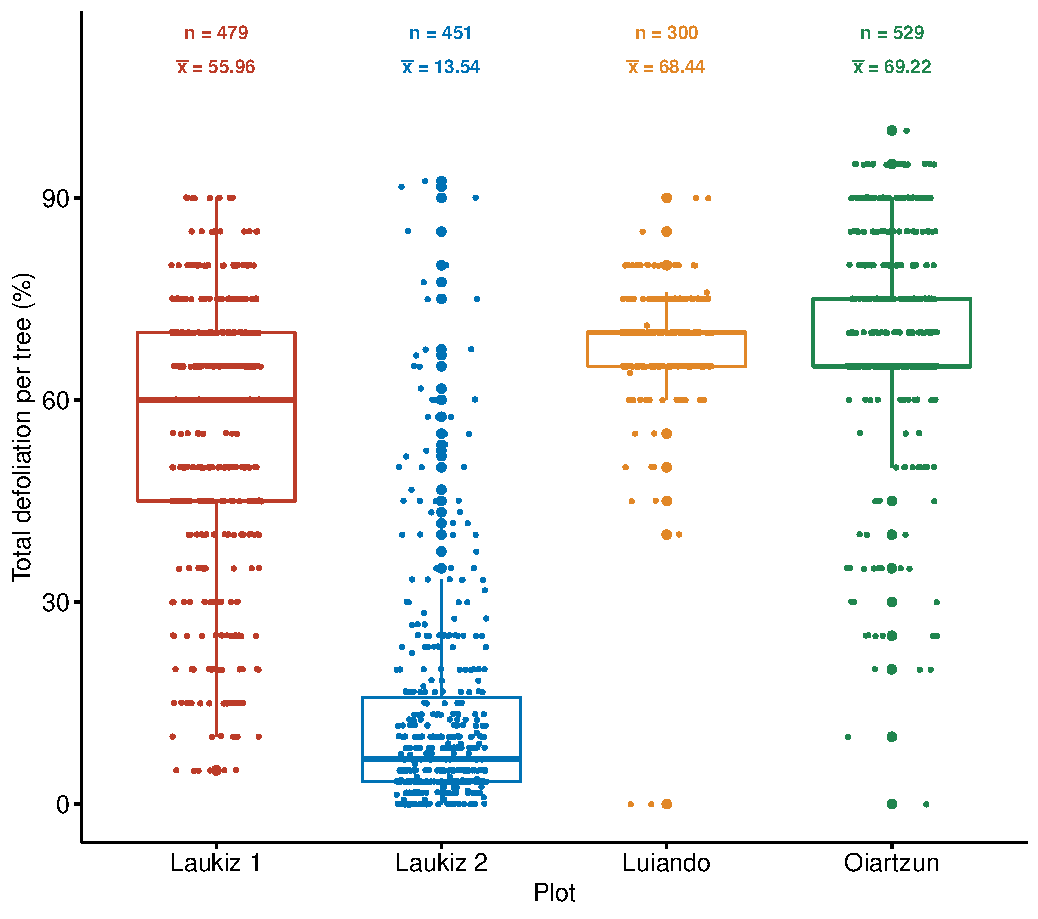
\includegraphics[width=0.7\textwidth] {defoliation-distribution-plot-1.pdf}}
\caption{Distribution of defoliation at trees for plots Laukiz 1, Laukiz 2, Luiando and Oiartzun.}
\label{fig:defol-distr}
\end{center}
\end{figure}



\subsection{In-situ data}

\noindent The \textit{Pinus radiata} plots of this study, namely \textit{Laukiz 1}, \textit{Laukiz 2}, \textit{Luiando} and \textit{Oiartzun}, are located in the northern part of the Basque Country (\autoref{fig:study_area}).
\textit{Oiartzun} has the most observations (n = 529) while \textit{Laukiz 2} features the largest area size (1.44 ha).
All plots besides \textit{Luiando} are located nearby the coast (\autoref{fig:study_area}).
In total 1759 observations are available (\textit{Laukiz 1} = 479, \textit{Laukiz 2} = 451, \textit{Luiando} = 300, \textit{Oiartzun} = 529).
The data was surveyed in September 2016.

\begin{figure} [t!]
	\begin{center}
		\makebox[\textwidth]{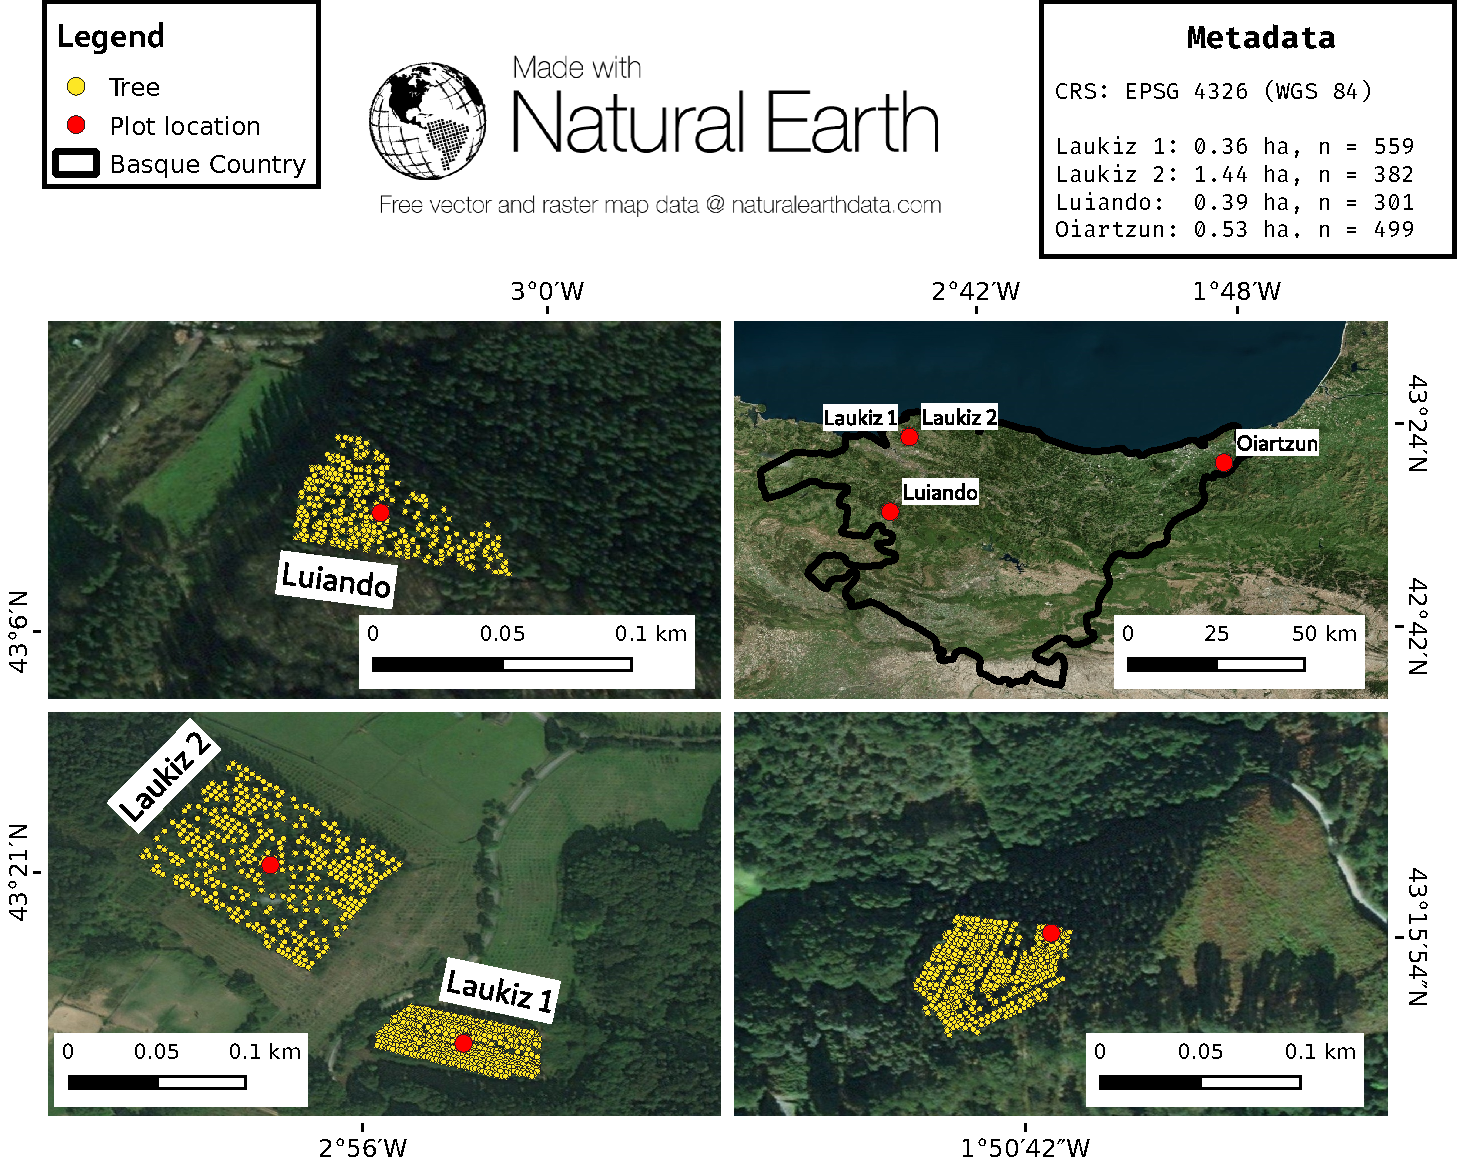
\includegraphics[width=\textwidth] {study_area_hyperspectral.pdf}}
		\caption{Information about location, size and spatial distribution of trees for all plots used in this study.}
		\label{fig:study_area}
	\end{center}
  \end{figure}


\subsection{Hyperspectral data}

\noindent The airborne hyperspectral data was acquired during two flight campaigns on September 28th and October 5th 2016, both around 12 am.
The images were taken using a AISAEAGLE-II sensor.
All preprocessing steps (geometric, radiometric, atmospheric) have been conducted by the \ac{ICGC}.
The first four bands are corrupted, leaving 122 bands with valid information.
Additional metadata information is available in \autoref{tab:hyperparameter_limits}.

% parameter limits
\begin{table}[b!]
\centering
\caption[t]{Specifications of hyperspectral data.}
\begingroup\footnotesize
\begin{tabular}{ll}
	\\
	Characteristic         & Value                               \\
	\hline
	Geometric resolution   & 1 m                                 \\
	Radiometric resolution & 12 bit                              \\
	Spectral resolution    & 126 bands (404.08 nm - 996.31 nm)   \\
	Correction:            & Radiometric, geometric, atmospheric
\end{tabular}
\endgroup
\label{tab:hyperparameter_limits}
\end{table}

\section{Methods}

\subsection{Derivation of indices}
% TODO: Mention different feature sets
\noindent To use the full information from the hyperspectral data, all possible vegetation indices supported by the R package \textit{hsdar} (90 in total) as well as all possible \ac{NRI} combinations were calculated.
The following formula was used for the NRI calculation:

\begin{equation}
	NRI_{i,j} = \frac{b_{i} - b_{j}}{b_{i} + b_{j}}
\end{equation}

\noindent
where $i$ and $j$ are the respective band numbers.

\bigbreak

\noindent To account for geometric offsets (which were reported with up to 1 m from \ac{ICGC}), a buffer of two meters around the centroid of the respective tree was used.
The mean of all pixels touched by this buffer was calculated and assigned to the observations.
In total, $\frac{125*126}{2} = 7875$ NRIs were calculated .
Due to four corrupted bands and numerical calculation errors for some band combinations, a total of 7471 indices were available for each observation.
All indices which contained missing values for at least one plot were removed from the dataset.
Observations were given more importance than indices due to the mass of available \ac{NRI} indices.

\subsection{Benchmarking design}

\noindent The benchmarking matrix of this study consists of the following algorithms:

\begin{itemize}
	\item  Extreme Gradient Boosting (XGBOOST)
	\item  Random Forest (RF)
	\item  Penalized Regression (both L1 and L2)
	\item  Support Vector Machine (SVM)
\end{itemize}


\noindent \ac{RF} and {SVM} are well established algorithms that are widely used in environmental modeling.
Extreme Gradient Boosting (commonly referred to as \ac{XGBOOST}) showed promising results in benchmark competitions in recent years.
Penalized Regression is a statistical modeling technique that is capable of dealing with highly-correlated covariates by applying a penalization term which shrinks the coefficients of the model \citep{hastie2001}.
The penalties are also known as "lasso" (L1) and "ridge" (L2).
The former does not allow the removal of variables from the model (penalization to zero) while the latter does.
Both penalties can also be combined.
The combined approach is called "elastic net" but was not used in this work.

\subsubsection{Feature sets}
% TODO: talk about the reasons behind different features sets: environmental implications

\noindent Three feature sets were used in this study with each representing a different way of feature-engineering:

\begin{itemize}
  \item The raw hyperspectal band information (HR): No feature engineering
  \item Vegetation Indices (\ac{VI}: Expert-based feature engineering
  \item Normalized Ratio Indices (\ac{NRI}): Automated feature-engineering
\end{itemize}

\subsubsection{Hyperparameter Optimization}

\noindent An exhaustive hyperparameter tuning was applied during nested spatial \ac{CV} for all algorithms.
Maximum Bayesian Optimization \citep{mlrmbo} was used for parameter optimization.
This approach first composes \textit{n} randomly chosen hyperparameter settings out of a user defined search space.
After these \textit{n} tries have been evaluated, a new hyperparameter setting, which is going to be evaluated next, is proposed based on a fitted regression model.
The regression model estimates the performance of the machine-learning method for unknown hyperparameter settings.
Using these estimates, a new promising hyperparameter setting is proposed to be evaluated next.
This strategy continues until a termination criterion, defined by the user, is reached \citep{hutter2011, jones1998}.
An initial design of 30 randomly composed hyperparameter settings and a termination criterion of 70 iterations was used, resulting in a total budget of 100 evaluated hyperparameter settings per fold.
The advantage of this tuning approach is the substantial reduction of the tuning budget required to find a setting which is close to the global minimum
This applies when being compared to methods that do not use information from previous runs, such as random search or grid search \citep{bergstra2012}.

\subsubsection{Spatial resampling}


\noindent A spatial block nested cross-validation was chosen to reduce the influence of spatial autocorrelation as much as possible.
Each plot served as one fold within the resampling setup, resulting in four folds total.
For the inner level (hyperparameter tuning), $p - 1$ folds were used (with $p$ being the number of plots). REF SCHRATZ

\subsection{Dimension reduction}

\noindent It is important to distinguish the term "dimension reduction" from "high-dimensionality".
The former refers to the general idea of reducing features from a dataset \citep{vandermaaten2007}.
In modeling this means finding the best subset of covariates which provide the most predictive power to the model.
The latter term in contrast is the definition of a dataset attribute:
When $p > n,$ where $p$ is the number of covariates and $n$ the number of observations \citep{hastie2001}, the dataset qualifies as "high-dimensional".
There is no absolute value at which the term can be applied, both for $n$ and $p$.
Hence for this study the word "high-dimensionality" only applies to the experiments using the "NRI" feature set (7470 features for 1759 observations).

The case of a feature-rich dataset comes with several challenges for both model fitting and evaluation.

\begin{itemize}
	\item Fitting times of the model increase
	\item Noise is possibly introduced into the model by highly-correlated variables \citep{johnstoneiainm.2009}
	      % I think we can phrase this better
	\item Interpretation and prediction becomes more complex, up to the point at which it is not possible anymore \citep{johnstoneiainm.2009}
\end{itemize}

\noindent In the last decade the amount of environmental data increased a lot, paramount by the increased data coverage of satellites.
With this the need of applying automated feature-selection methods emerged.
In the following sections the currently most used feature selection approaches are briefly introduced.

\subsubsection{Filter methods}

% Filter methods
\noindent The concept of "Filter methods" originates on the idea of ranking features using certain heuristics of an algorithm \citep{chandrashekar2014}.
Some filter methods are restricted towards specific types of variables (numeric or nominal data).
After the covariates have been ranked, a decision needs to be made what features to keep and which to discard \citep{drotar2015}.
This step is usually done within the optimization phase of the model fitting, along with the hyperparameter tuning.
Essentially, the number of covariates in the model is treated as a hyperparameter of the model.
The goal is to optimize the number of features (using the ranked covariates) at which the model achieves the best performance.
In well-implemented software solutions the filter calculation is only done once and then cached, saving valuable resources \citep{mlr}.

% Ensemble filter methods
Besides the concept of choosing a specific filter method to rank variables, studies showed that combining several filters using statistical operations such as "minimum", "mean" or "sum" are able to enhance the predictive performance of the resulting models \citep{abeel2010, drotar2017a}.
This aligns with the recent rise of the "ensemble" approach in machine-learning which uses stacking to combine the predictions of multiple models \citep{polikar2012, feurer2015}.
In this work the "Borda" ensemble filter was applied \citep{drotar2017a}.
Here, the ranking is based on the sum of all single filters.

Most filter methods are correlation or entropy based.
A list of all filter methods used in this work along with their respective formulas can be found in Appendix X.
% TODO: Link appendix
% TODO: List filter methods

% I grouped these two since we focus on filter methods in this study - or is this already a bit biased towards filter methods?
\subsubsection{Other approaches}

% Wrapper approach
\noindent Another approach to reduce the number of variables is to apply algorithms that are used for hyperparameter optimization such as "Random Search" or a "Generic Simulated Annealing".
First a (random) subset of features is chosen based on the selected algorithm.
In comparison to "filters", no ranking is applied in this step.
Now the model is fitted on the data and the performance is evaluated.
A disadvantage of this approach is that hyperparameter tuning can only start after the feature-selection optimization has ended.
Hence, this method is very expensive because two optimization stages need to be run.
In science this approach is also referred to as "wrapper method" \citep{chandrashekar2014, kohavi1997}.
It was not considered in this work due to the expensive runtime.

% PCA
A third commonly used method is the "Principal Component Analysis" \citep{pearson1901, jolliffe2016}.
Here, the main components of the feature space are extracted and combined.
Usually the first two components are taken since these contain the major information of the covariates.
By using the (automatically estimated) explained variance of the main components, the model can rely on a few features containing the majority of information available in the data.
This enables a very cheap model fitting with a minimal loss of predictor information.
However, the resulting features used in the model do not relate anymore to the raw input variables since they are a combination of multiple covariates.
Interpretation is not possible anymore.

\noindent The complete study was done using the open-source statistical programming language R \citep{rcoreteam2018}.
The algorithm implementations of the following packages have been used: \textit{xgboost} \citep{chen2016} (\textit{xgboost}), \textit{e1071} \citep{e1071} (Support Vector Machine) and \textit{glmnet} \citep{glmnet} (Ridge Regression).
The filter methods of the following packages were used: \textit{praznik \citep{praznik}}, \textit{FSelectorRcpp} \citep{fselectorrcpp}.
The R package \textit{mlr} \citep{mlr} was used for all modeling related steps.
\textit{drake} was used for structuring the work and ensuring reproducibility.
This study is available as a research compendium on Zenodo (\url{10.5281/zenodo.2635403}).



\section{Results}

\subsection{Predictive performance}


\section{Discussion}

\subsection{Derivation of indices}

\noindent The decision to use a buffer of 2 m to generate the index value for each observation is questionable.
When using no buffer at all, the possibility is high that a pixel value gets assigned to the tree observation which does not spatially match with the hyperspectral (due to the geometric offset of 1 m).
Using a buffer of more than 2 meters would increase the probability of merging information from other trees into the pixel value, blurring the actual value of the tree observation.
That is why in our view using a buffer of 2 m was the best compromise here.

Another critical point is that the exact number of contributing pixels to the final index value of an observation cannot be determined as it depends on the location of the tree within the pixel grid.
As the buffer is a circle, it depends on the exact location of a tree observation within a pixel how much surrounding pixels are touched by the buffer.
If a tree observation is located at the border of the plot, some directions of the buffer will contain no values and the subsequent index value will be calculated using less pixels than if the tree observation is located in the middle of the plot.

All these points introduced a bias of an unknown magnitude into the data.
This has to be considered when making interpretations about the outcome of this study.

\subsection{Performance vs. plot characteristics}

\subsection{Predictive Performance}

\subsubsection{Algorithm benchmarking}

\subsection{Feature selection methods}

\subsection{Comparison to other studies}A
% NOTE: no environmental studies use filter methods, some use FFS
% NOTE: only few studies analyze defoliation

\noindent Most other studies analyzing defoliation operated on the plot rather than the tree level.
This originated simply due to spatial resolution of the satellite products that served as the input data \citep{townsend2012, debeurs2008a, rengarajan2016}.

Studies focusing on tree-level defoliation used ground-level methods such as \ac{ALS} or \ac{LiDAR} \citep{meng2018, kalin2019}.
\cite{meng2018} used \ac{OLS} regression methods while \cite{kalin2019} retrieved information out of ground-level RGB photos using \ac{CNN}.
Both study designs are substantially different compared to the setup of this work.
In addition, no spatial \ac{CV} or \ac{FS} was used.
\cite{goodbody2018} used a \ac{PLS} model with high-resolution \ac{DAP} to predict cumulative defoliation caused by the spruce budworm.
Study results indicated that spectral metrics were found to be most helpful for the model.
Incorporating such metrics (both spectral and structural) could be a possible enhancement for future works.

\cite{shendryk2016, ludwig2019} are studies which are more similar in their methodology but focus on a different response variable.
\cite{shendryk2016} used machine-learning models with \ac{ALS} data to study dieback of trees for eucalyptus forests.
A grid-search was used for hyperparameter tuning and a \ac{FFS} for variable selection.
\cite{ludwig2019} analyzed woody cover in South Africa using spatial \ac{CV} and a relatively novel spatial \ac{FS} approach \citep{meyer2018} on a Random Forest classifier.


In summary, we could not find studies using filter methods for \ac{FS} or \ac{NRI} indices in their work with a relation to forest health.
Most studies used only one algorithm (usually Random Forest) without strong arguments why this particular one has been selected.
In our view the number of possible derivable input features is often higher than the number of variables used in the end, missing out potential helpful information from the data.
These findings underline the importance of this work in the field of forest health modeling.

\section{Outlook and conclusion}

\noindent In this work we used various indices derived from hyperspectral remote sensing data to estimate defoliation as a proxy for tree health in northern Spain.
In the algorithm comparison \textit{xgboost} showed the best performance among the tested ones.
Even though \ac{RR} is able to handle highly correlated data, it was far from achieving an acceptable performance in this work.

The fitted models on the plot level showed a promising performance with RMSE values between 8 and 20 which validated the approach of relating defoliation to remote sensing indices.
The performance of the model containing all data (four plots) was acceptable (RMSE 29.59) but can be improved by adding more observations from other plots in future studies.

The spatial prediction showed a satisfying result making it possible to distinguish highly defoliated plots from plots with low defoliation easily.
The most important indices for the fitted model were widely known vegetation indices such as EVI, GDVI or NDVI.
In future studies it would be interesting to link the indices of this work to other indicators of forest/vegetation health and analyze their importance and the model performances.

\section{Appendix}

\appendix
% https://tex.stackexchange.com/questions/248704/cross-reference-to-appendix-sections-in-elsarticle-document-class
\gdef\thesection{\Alph{section}} % corrected redefinition of "\thesection"
\makeatletter
\renewcommand\@seccntformat[1]{Appendix \csname the#1\endcsname.\hspace{0.5em}}
\makeatother

\section{Spectral signatures of each plot}

% spectral signatures
%\begin{figure} [H]
%\begin{center}
%\makebox[\textwidth]{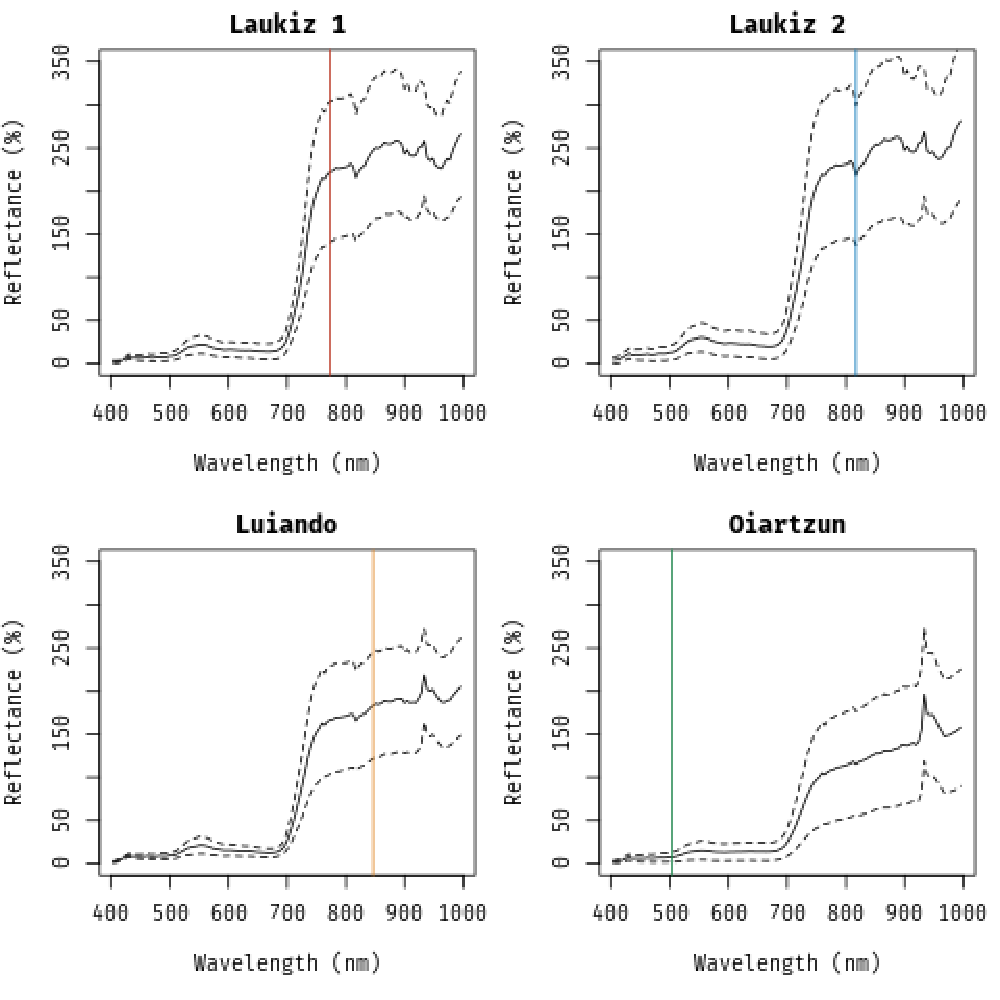
\includegraphics[width=\textwidth] {spectral_signatures.pdf}}
%\caption{Spectral signatures (mean and standard deviation) of each plot.}
%\label{fig:spectral_signatures}
%\end{center}
%\end{figure}

\pagebreak


\section*{References}

\bibliography{Biblio}

\end{document}

